\let\lesson\undefined
\newcommand{\lesson}{\phantomlesson{Bài 10: Tổng hợp lực và phân tích lực. Cân bằng lực}}
\chapter[Tổng hợp lực và phân tích lực. Cân bằng lực]{Tổng hợp lực và phân tích lực. Cân bằng lực}
\setcounter{section}{0}
\section{Lý thuyết}
\subsection{Lực}
\begin{itemize}
	\item Lực là đại lượng vectơ đặc trưng cho tác dụng của vật này lên vật khác mà kết quả là gây ra gia tốc cho vật hoặc làm cho vật biến dạng.
	\item Đơn vị của lực trong hệ SI là newton (N).	
\end{itemize}
\subsection{Tổng hợp lực}
Tổng hợp lực là thay thế các lực tác dụng đồng thời vào cùng một vật bằng một lực có tác dụng giống hệt như hệ các lực ấy.

\subsubsection{Cách xác định hợp lực}
Hợp lực $\vec{F}=\vec{F}_1+\vec{F}_2$ của hai lực đồng quy $\vec{F}_1$ và $\vec{F}_2$ được xác định như sau
\begin{itemize}
	\item độ lớn 
	\begin{align*}
		F=\sqrt{F_1^2+F_2^2+2F_1F_2\cos \alpha},
	\end{align*}
	trong đó, $\alpha$ là góc hợp bởi vectơ $\vec{F}_1$ và $\vec{F}_2$.
	\item điểm đặt trên vật, cũng là điểm giao của hai lực $\vec{F}_1$ và $\vec{F}_2$.
	\item phương của $\vec{F}$ được xác định theo quy tắc hình bình hành: $\vec{F}$ được biểu diễn bởi đường chéo của hình bình hành như Hình \ref{fig:14.1}. Khi này gốc của hai vectơ lực thành phần phải trùng nhau.
	\begin{center}
		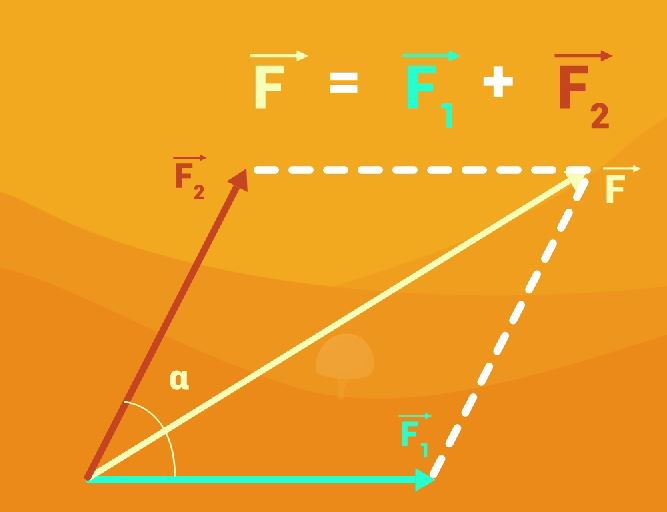
\includegraphics[scale=0.35]{../figs/VN10-PH-11-L-008-2-V2-01.jpg}
		\captionof{figure}{Minh hoạ cách tổng hợp lực bằng quy tắc hình bình hành.}
		\label{fig:14.1}
	\end{center}
\end{itemize}
\manatip{
	Độ lớn hợp lực trong một số trường hợp đặc biệt:
	\begin{itemize}
		\item Nếu $\vec{F}_1$ cùng chiều $\vec{F}_2$ $$F=F_1+F_2,$$
		\item Nếu $\vec{F}_1$ ngược chiều $\vec{F}_2$ $$F=|F_1-F_2|,$$
		\item Nếu $\vec{F}_1$ vuông góc $\vec{F}_2$ $$F=\sqrt{F_1^2+F_2^2}.$$
	\end{itemize}
}
Ngoài ra, người ta cũng có thể tổng hợp lực bằng các quy tắc sau:
\begin{itemize}
	\item Quy tắc tam giác lực: Ta có thể tịnh tiến vectơ lực $\overrightarrow{F_2}$ sao cho gốc của nó trùng với ngọn của vectơ lực $\overrightarrow{F_1}$ như (Hình \ref{fig:14.2}a). Khi này, vectơ lực tổng hợp $\vec{F}$ là vectơ nối gốc của $\overrightarrow{F_1}$ với ngọn của vectơ $\overrightarrow{F_2}$.
	\item Khi vật chịu tác dụng của nhiều hơn hai lực. Ta có thể áp dụng một cách liên tiếp quy tắc tam giác lực để tìm hợp lực. Quy tắc này gọi là quy tắc đa giác lực (Hình \ref{fig:14.2}b).
	\begin{center}
		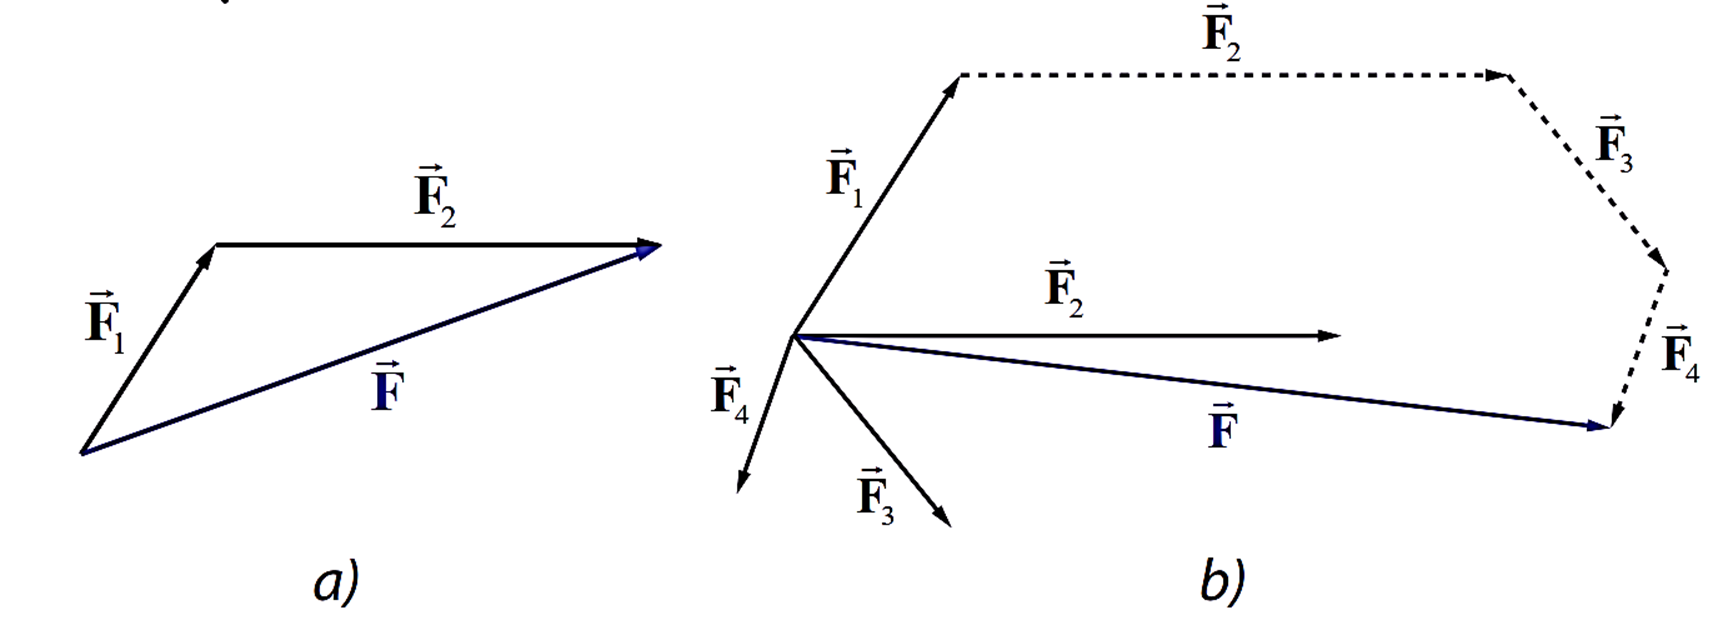
\includegraphics[width=0.7\linewidth]{../figs/VN10-2023-PH-TP014-2}
		\captionof{figure}{Minh hoạ cách tổng hợp lực bằng: 
		\textit{a) quy tắc tam giác lực; b) quy tắc đa giác lực}}
		\label{fig:14.2}
	\end{center}
\end{itemize}
\subsection{Điều kiện cân bằng lực}
Muốn cho một chất điểm đứng cân bằng thì hợp lực của các lực tác dụng lên nó phải bằng không.
$$\vec{F}=\vec{F}_1+\vec{F}_2+...=\vec{0}.$$
\subsection{Phân tích lực}
\begin{itemize}
	\item Phân tích lực là thay thế một lực bằng hai hay nhiều lực có tác dụng giống hệt như lực đó.
	\item Phân tích lực là phép làm ngược lại với tổng hợp lực. Phân tích một lực thành hai lực thành phần đồng quy phải tuân theo quy tắc hình bình hành. 
\end{itemize}
Thông thường, người ta phân tích lực thành hai lực thành phần vuông góc với nhau để lực thành phần này không có tác dụng nào theo phương của lực thành phần kia.
\begin{center}
	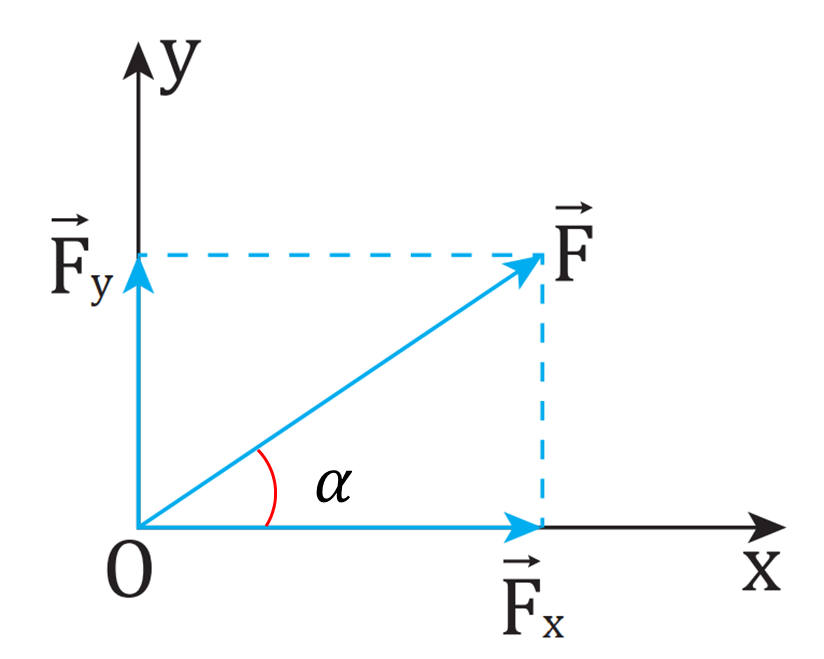
\includegraphics[width=0.25\linewidth]{../figs/VN10-2023-PH-TP014-3}
	\captionof{figure}{Phân tích lực $\vec{F}$ thành hai lực thành phần vuông góc $\overrightarrow{F_x}$ và $\overrightarrow{F_y}$.}
\end{center}
Nếu gọi $\alpha=\left(\overrightarrow{F}, \overrightarrow{F_x}\right)$ thì 
\begin{align*}
	\begin{cases}
		F_x=F\cos\alpha\\
		F_y=F\sin\alpha
	\end{cases}
\end{align*}
\section{Mục tiêu bài học - Ví dụ minh họa}
\begin{dang}{Ghi nhớ đặc điểm hợp lực của  hai lực đồng quy}
	\viduii{1}{Một chất điểm chịu tác dụng đồng thời của hai lực thành phần có độ lớn $F_1$ và $F_2$ thì hợp lực $\vec{F}$ của chúng luôn có độ lớn thỏa mãn hệ thức: 
		\begin{mcq}(2)
			\item $F = F_1^2 +F_2^2$.
			\item $|F_1 - F_2 |\leq F \leq F_1 +F_2.$
			\item $F = F_1+F_2.$
			\item $F = \sqrt {F_1^2+F_2^2}.$
		\end{mcq}
	}
	{	\begin{center}
			\textbf{Hướng dẫn giải}
		\end{center}
		
		Về độ lớn $|F_1-F_2|\leq F\leq F_1+F_2.$
		
		\textbf{Đáp án: B}.
	}
	\viduii{1}{Lực tổng hợp của hai lực đồng quy có giá trị lớn nhất khi 
		\begin{mcq}(2)
			\item Hai lực thành phần cùng phương, cùng chiều.      
			\item Hai lực thành phần cùng phương, ngược chiều.
			\item Hai lực thành phần vuông góc với nhau. 
			\item Hai lực thành phần hợp với nhau một góc khác không.
		\end{mcq}
	}
	{	\begin{center}
			\textbf{Hướng dẫn giải}
		\end{center}
		
		Hai vectơ cộng nhau tạo thành một vectơ có độ lớn cực đại khi hai vectơ đó cùng chiều với nhau. 
		
		
		\textbf{Đáp án: A}.
	}
\end{dang}

\begin{dang}{Tổng hợp lực \\theo quy tắc hình bình hành. }
	\viduii{2}{Tìm độ lớn hợp lực $\vec F$ của hai lực đồng quy $\vec{F}_1$ và $\vec{F}_2$ trong các trường hợp sau, nếu biết độ lớn $F_1=\SI{30}{N}$, $F_2=\SI{40}{N}$, góc giữa $\vec{F}_1$ và $\vec{F}_2$ là:
		\begin{enumerate}[label=\alph*.]
			\item $\alpha =0^\circ$.
			\item $\alpha =60^\circ$.
			\item $\alpha =90^\circ$.
			\item $\alpha =180^\circ$.
		\end{enumerate}
	}
	{	\begin{center}
			\textbf{Hướng dẫn giải}
		\end{center}
		
		\begin{enumerate}[label=\alph*.]
			\item Góc hợp bởi $\vec{F}_1$ và $\vec{F}_2$ là $\alpha =0^\circ$, tức là  $\vec{F}_1$ cùng chiều $\vec{F}_2.$
			
			Do đó, độ lớn $F=F_1+F_2= 70\, \si{\newton}$.
			\item Góc hợp bởi $\vec{F}_1$ và $\vec{F}_2$ là $\alpha =60^\circ.$
			
			Do đó, độ lớn $F=\sqrt{F_1^2+F_2^2+2F_1F_2\cos \alpha }= 10\sqrt{37}\,\si{\newton}$.
			\item Góc hợp bởi $\vec{F}_1$ và $\vec{F}_2$ là $\alpha =90^\circ$, tức là  $\vec{F}_1$ vuông góc $\vec{F}_2.$
			
			Do đó, độ lớn $F=\sqrt{F_1^2+F_2^2}=50\, \si{\newton}$.
			\item Góc hợp bởi $\vec{F}_1$ và $\vec{F}_2$ là $\alpha =180^\circ$, tức là  $\vec{F}_1$ ngược chiều $\vec{F}_2.$
			
			Do đó, độ lớn $F=|F_1-F_2|= 10\si{\newton}$.
		\end{enumerate}
		
	}
	\viduii{2}{Cho hai lực đồng quy có cùng độ lớn $\SI{9}{N}$. Góc giữa hai lực bằng bao nhiêu thì hợp lực cũng có độ lớn bằng $\SI{9}{N}$? 
	}
	{	\begin{center}
			\textbf{Hướng dẫn giải}
		\end{center}
		
		Độ lớn:
		$$F=\sqrt{F_1^2+F_2^2+2F_1F_2\cos \alpha }.$$
		$$\Rightarrow \cos \alpha = \dfrac{F^2-F_1^2-F_2^2}{2F_1F_2}= -\dfrac{1}{2}.$$
		$$\Rightarrow \alpha =120^\circ. $$
		
		Vậy góc giữa hai lực bằng $120^\circ.$
	}
\end{dang}
\begin{dang}{Ghi nhớ đặc điểm của phép phân tích lực}
	\viduii{1}{Khi nói về phép phân tích lực, phát biểu nào sau đây đúng?
		\begin{mcq}
			\item Phân tích lực là thay thế một lực bằng hai hay nhiều lực có tác dụng giống hệt như lực đó.
			\item Khi phân tích một lực thành hai lực thành phần thì phải tuân theo quy tắc tam diện thuận.
			\item Khi phân tích một lực thành hai lực thành phần thì hai lực thành phần làm thành hai cạnh của tam giác.
			\item Phân tích lực là phép thay thế các lực tác dụng đồng thời vào vật bằng một lực như các lực đó.
		\end{mcq}
	}
	{	\begin{center}
			\textbf{Hướng dẫn giải}
		\end{center}
		
		Phân tích lực là thay thế một lực bằng hai hay nhiều lực có tác dụng giống hệt như lực đó.Các lực thay thế gọi là các lực thành phần. 
		
		A - đúng
		
		B – sai vì: Khi phân tích một lực thành hai lực thành phần thì phải tuân theo quy tắc hình bình hành
		
		C – sai vì chưa đầy đủ vị trí của hai cạnh này so với lực ban đầu.  
		
		D – sai, đây là phép tổng hợp lực. 
		
		\textbf{Đáp án: A}.
	}
	\viduii{1}{Điều nào sau đây là đúng khi nói về phép phân tích lực. 
		\begin{mcq}
			\item Phép phân tích lực là phép làm ngược lại với phép tổng hợp lực. 
			\item Phép phân tích lực tuân theo qui tắc hình bình hành.
			\item Phép phân tích lực là phép thay thế một lực bằng hai hay nhiều lực thành phần.   
			\item Cả A, B và C đều đúng.
		\end{mcq}
	}
	{	\begin{center}
			\textbf{Hướng dẫn giải}
		\end{center}
		
		Phân tích lực là thay thế một lực bằng hai hay nhiều lực có tác dụng giống hệt như lực đó. Các lực thay thế gọi là các lực thành phần. 
		
		\textbf{Đáp án: D}.
	}
\end{dang}

\begin{dang}{Phân tích lực theo quy tắc hình bình hành}
	\viduii{2}{Một chất điểm chịu tác dụng đồng thời của hai lực thành phần vuông góc với nhau có độ lớn lần lượt là $F_1 = \SI{15}{N}$ và $F_2$. Nếu hợp lực có độ lớn là $\SI{25}{N}$ thì giá trị của $F_2$ là
		\begin{mcq}(4)
			\item $\SI{10}{N}$.
			\item $\SI{20}{N}$.
			\item $\SI{30}{N}$.
			\item $\SI{40}{N}$.
		\end{mcq}
	}
	{	\begin{center}
			\textbf{Hướng dẫn giải}
		\end{center}
		
		Nếu $\vec{F}_1$ vuông góc $\vec{F}_2$ thì hợp lực sẽ có độ lớn 
		$$F=\sqrt{F_1^2+F_2^2} \quad\Rightarrow\quad F_2=\sqrt{F^2-F_1^2}.$$
		
		Thay các giá trị từ đề bài, độ lớn hợp lực có giá trị 		
		$$F_2 = \sqrt {F^2 - F_1^2} =\sqrt{(\SI{25}{\newton})^2-(\SI{15}{\newton})^2}= \SI{20}{N}.$$
		
		\textbf{Đáp án: B}.
	}
	\viduii{2}{Cho lực $F$ có độ lớn $\SI{100}{N}$ và có hướng tạo với trục Ox một góc $\SI{36,87}{^\circ}$. Xác định độ lớn các thành phần của lực $F$ trên các trục Ox và Oy.
	}
	{	\begin{center}
			\textbf{Hướng dẫn giải}
		\end{center}
		
		%		Độ lớn của góc hợp bởi Ox và Oy
		
		%		$$\SI{36,87}{^\circ} + \SI{53,13}{^\circ}= \SI{90}{^\circ}$$
		
		Độ lớn các thành phần của lực $F$
		\begin{align*}
			F_{x} &= F\cos \SI{36,87}{^\circ} = \SI{80}{N}\\
			F_{y}&= F\sin\SI{36,87}{^\circ} = \SI{60}{N}
		\end{align*}
	}
\end{dang}

